%=================================================================
% EJEMPLO -- Equipo 0 (equipo ficticio de la plantilla), segundo corte.
% Version REVISADA del paper despues de las observaciones del primer
% corte. Las marcas \linelabel{ln:...} y \label{...} son las que lee la
% respuesta a los revisores ("../Equipo 0 - respuesta - segundo corte").
% Compilar: pdflatex -> bibtex -> pdflatex -> pdflatex.
%=================================================================
\documentclass[lettersize,journal]{IEEEtran}

\usepackage{amsmath,amsfonts}
\usepackage{array}
\usepackage{textcomp}
\usepackage{url}
\usepackage{graphicx}
\usepackage{cite}
\usepackage{xcolor}
\usepackage{tikz}
\usetikzlibrary{positioning,arrows.meta}
\usepackage{balance}

\begin{document}

\title{A Load-Cell Cup Detection Module for the RoboCoffee Delivery Fleet}

\author{Student~A, Student~B, Student~C, Jorge~A.~Lizarraga and Graciela~Baca
\thanks{The authors are with the Department of Technological and
Industrial Processes, ITESO, Tlaquepaque 45604, Jalisco, Mexico.}}

\markboth{LabDST RoboCoffee, ITESO, Fall 2026}%
{Student \MakeLowercase{\textit{et al.}}: Load-Cell Cup Detection for RoboCoffee}

\maketitle

\begin{abstract}
\linelabel{ln:abs}This paper presents a cup detection module for the RoboCoffee intralogistics fleet. The module measures the load on the cup holder with a strain-gauge load cell and reports placement and removal events to the central platform. A threshold rule with hysteresis is proposed, and a preliminary test of 20 placement--removal cycles is reported.
\end{abstract}

\begin{IEEEkeywords}
Service robots, intralogistics, load cell, object detection, mobile robots.
\end{IEEEkeywords}

%=================================================================
\section{Introduction}
\label{sec:intro}

% \linelabel va DENTRO del texto del parrafo (despues de \IEEEPARstart), nunca
% antes ni entre parrafos: ahi lineno crea una linea vacia numerada y la
% referencia apunta a esa linea vacia.
\IEEEPARstart{D}{ifferential-drive} \linelabel{ln:intro-p1}mobile robots are a mature platform for indoor service tasks, since their kinematics and odometry are well understood \cite{siegwart2011autonomous}. In a coffee-delivery service, however, the robot must also know whether the order is still on board: a delivery is only complete when the client removes the cup.

\linelabel{ln:intro-fleet}When several robots share the same pool of orders, the waiting time of each client depends on how quickly a robot is released after each delivery, which can be analyzed with queueing models \cite{kleinrock1975queueing}. \linelabel{ln:intro-cite}A robot that cannot confirm the removal of the cup either waits a fixed time, which wastes fleet capacity, or leaves too early, which risks returning with an undelivered order.

\linelabel{ln:rq}This work addresses the following research question: can a single
load cell under the cup holder detect cup placement and removal reliably enough, and
fast enough, to release the robot automatically at the end of each delivery?

\linelabel{ln:contrib}The contributions of this paper are: (i) a low-cost detection
module that uses a load cell and an ESP32 microcontroller; (ii) a threshold rule
with hysteresis that rejects the vibration produced while the robot moves; and (iii)
a test protocol that quantifies detection reliability and
latency.\linelabel{ln:contrib-end}

%=================================================================
\section{Related Work}
\label{sec:related}

\linelabel{ln:rw-rfid}Radio-frequency identification (RFID) is a common way to detect tagged objects \cite{want2006rfid}. \linelabel{ln:rw-bench}However, RFID requires a tag on every cup, which is not compatible with the disposable cups used in a cafeteria. Measuring the weight of the cup does not require any tag and also distinguishes an empty holder from a full or an empty cup.\linelabel{ln:rw-end}

%=================================================================
\section{Materials and Methods}
\label{sec:methods}

\linelabel{ln:mm-arch}The architecture of the module is shown in Fig.~\ref{fig:arch}. A 1\,kg strain-gauge load cell supports the cup holder; an HX711 amplifier converts its signal at 80\,Hz, and an ESP32 applies the detection rule and sends events to the central platform over Wi-Fi.\linelabel{ln:mm-arch-end}

\begin{figure}[!t]
\centering
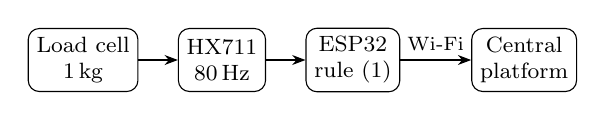
\begin{tikzpicture}[node distance=4mm and 5mm,
  box/.style={draw, rounded corners, align=center, font=\footnotesize,
              minimum height=8mm, inner sep=3pt},
  >={Stealth}]
\node[box] (lc) {Load cell\\1\,kg};
\node[box, right=of lc] (hx) {HX711\\80\,Hz};
\node[box, right=of hx] (esp) {ESP32\\rule (1)};
\node[box, right=9mm of esp] (pf) {Central\\platform};
\draw[->] (lc) -- (hx);
\draw[->] (hx) -- (esp);
\draw[->] (esp) -- node[above, font=\scriptsize]{Wi-Fi} (pf);
\end{tikzpicture}
\caption{Architecture of the cup detection module.}
\label{fig:arch}
\end{figure}

\linelabel{ln:mm-rule}Let $m_k$ be the filtered mass at sample $k$. The state $s_k$ of the holder changes only when the mass crosses one of two thresholds:
\begin{equation}
s_k=\begin{cases}
1, & m_k > m_{\mathrm{on}},\\
0, & m_k < m_{\mathrm{off}},\\
s_{k-1}, & \text{otherwise},
\end{cases}
\label{eq:rule}
\end{equation}
\linelabel{ln:mm-thr}with $m_{\mathrm{on}}=40$\,g and $m_{\mathrm{off}}=20$\,g. The gap between both thresholds prevents false events caused by the vibration of the holder while the robot moves.\linelabel{ln:mm-thr-end}

\linelabel{ln:mm-protocol}The test protocol is summarized in Table~\ref{tab:protocol}. Each cycle consists of placing a cup, moving the robot 3\,m, and removing the cup; the latency is the time between the removal and the event received by the platform.\linelabel{ln:mm-protocol-end}

\begin{table}[!t]
\caption{Test protocol}
\label{tab:protocol}
\centering
\begin{tabular}{|l|l|}
\hline
Cups tested & empty (12\,g), full (250\,g) \\
\hline
Cycles & 20 (this cut), 100 (next cut) \\
\hline
Metrics & detection rate, false events, latency \\
\hline
\end{tabular}
\end{table}

%=================================================================
\section{Preliminary Results}
\label{sec:results}

\linelabel{ln:res-trials}In the 20 preliminary cycles with a full cup, all placements and removals were detected and no false events occurred while the robot was moving. The mean removal latency was 0.31\,s. These results correspond to a single cup type and a single robot; the complete campaign of 100 cycles with both cup types will be reported in the next cut.\linelabel{ln:res-end}

%=================================================================
\section{Discussion and Limitations}
\label{sec:discussion}

\linelabel{ln:disc-empty}An empty disposable cup (12\,g) lies below
$m_{\mathrm{off}}$, so the current rule cannot distinguish an empty cup from an
empty holder. \linelabel{ln:disc-vision}Camera-based detection could identify the
cup independently of its weight, but it would add an image-processing pipeline and
lighting requirements outside the scope of this module; it is therefore left as
future work.\linelabel{ln:disc-end}

%=================================================================
\section{Conclusions}
\label{sec:conclusions}

\linelabel{ln:concl}A load-cell module with a hysteresis rule detected cup placement and removal in all preliminary cycles with a sub-second latency, which supports its use to release RoboCoffee robots automatically after each delivery.

\bibliographystyle{IEEEtran}
\bibliography{bibliography}

\end{document}
